\documentclass[conference,compsoc]{IEEEtran}
\usepackage{./macros}

\begin{document}
\title{CS5300 Assignment 5\\Designing and Implementing Lock-Based Savings Account}
\author{Gautam Singh\\CS21BTECH11018}
\maketitle
\tableofcontents

\bigskip

\begin{abstract}
    This report describes the design of a mutithreaded lock-based savings
    account in C++ that supports deposit and withdraw options. Additionally,
    there are two types of withdraws: ordinary and preferred, with the latter
    type of withdrawal having priority over the former. We analyze the
    throughput and latency of this implementation in various situations.
    Finally, we document some challenges faced during the implementation.
\end{abstract}

\section{Program Design}
\label{sec:prog-design}

We give here an overview of the implementation details of the program.

\subsection{Savings Account}
\label{subsec:snap-interface}

The savings account object is implemented as a C++ class, following the
interface given in \autoref{code:savings-account}.

\begin{listing}[!ht]
\inputminted{cpp}{codes/SavingsAccount.cpp}
\caption{C++ SavingsAccount interface.}
\label{code:savings-account}
\end{listing}

We have one lock per account and two condition variables on that lock. The
\texttt{preferredCondition} condition variable checks if there is a preferred
withdrawal already waiting (except for the current thread). Threads check this
by reading the value of \texttt{preferredWaiting}. On the other hand, the
\texttt{balanceCondition} condition variable checks if the account has enough
balance for withdrawal.

\subsection{Threads and Runner Functions}
\label{subsec:threads-and-runners}
Threads are created using the C++ \texttt{std::thread} class. This makes it
convenient to pass thread IDs and references to other objects using
\texttt{std::ref} to the thread runner functions. In particular, we pass the
following arguments to the runner function.

\begin{enumerate}
    \item Thread ID from 0 to \(N - 1\), where \(N\) is the number of threads.
    This is because the \texttt{std::thread} class creates threads with IDs that
    may not be in this range, as they are only meant to be unique. However,
    these IDs are only used in logging and not in the snapshot algorithms.
    \item Logging output vector (a reference to a C++
    \texttt{std::vector<std::string>} object) to write timing information for
    further analysis and output. Our logs contain the (padded) time at the
    prefix, thus we can sort the logs directly.
\end{enumerate}

\subsection{Timing}
\label{subsec:timing}

The timestamps are reported using the \texttt{std::chrono} library. To prevent
zero values, we report times in nanoseconds, which is the smallest available
unit of time. However, results in the analysis are suitably scaled and reported
in milliseconds where needed.

\subsection{Random Number Generation}
\label{subsec:rng}

Random sleep times are generated using exponential distributions with a mean of
\(\alpha\) milliseconds. This is done using the
\texttt{std::exponential\_distribution} class. Further, the operation to be
performed and the balance for the operation (whether deposit or withdrawal) is
decided using uniform distributions. The randomness is generated using a
Mersenne Twister, instantiated using an \texttt{std::mt19937} object. This
random number generator is seeded using the current time since epoch.

\section{Results and Analysis}
\label{sec:results}

\subsection{Throughput vs. Number of Threads}

The scalability of our implementation is depicted in \autoref{fig:exp1}. In this
setting, we vary the number of threads instantiated and plot the throughput
curves for two sets of 10 and 50 accounts respectively. We observe the
following.

\begin{enumerate}
    \item The throughput is larger for the 50 account setting than the 10
    account setting. Further, the increase is pronounced for a larger number of
    threads. This is because the work among a larger number of accounts is
    divided equally into more threads. Thus, there are fewer chances of blocking
    since threads invoke methods on different accounts.
    \item The throughput in both cases decreases with increasing the number of
    threads. This might indicate more amount of blocking among threads when the
    number of threads increases, which is expected due to the higher
    competition. 
\end{enumerate}

\begin{figure}[!ht]
    \centering
    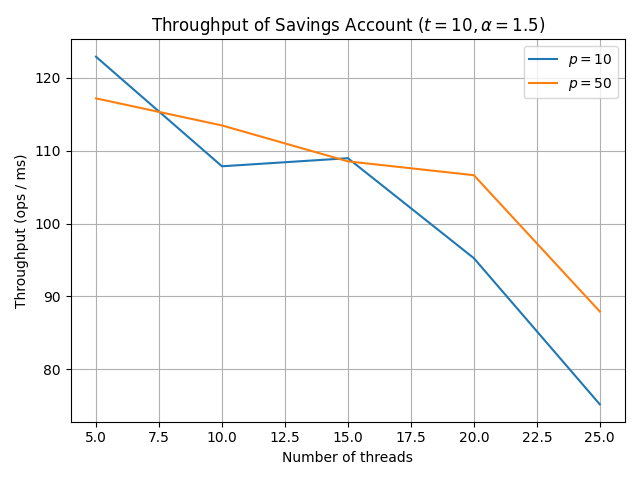
\includegraphics[width=\columnwidth]{images/exp1.png}
    \caption{Throughput vs. Number of Threads}
    \label{fig:exp1}
\end{figure}

\subsection{Latency vs. Number of Operations per Thread}

We now determine the latency of the savings account implementation by computing
the average latency for all operations. Since this is inversely related to the
throughput, we observe opposite trends here, as shown in \autoref{fig:exp2}.
Briefly, there are higher latencies for operating fewer number of accounts as
well as for larger number of threads.

\begin{figure}[!ht]
    \centering
    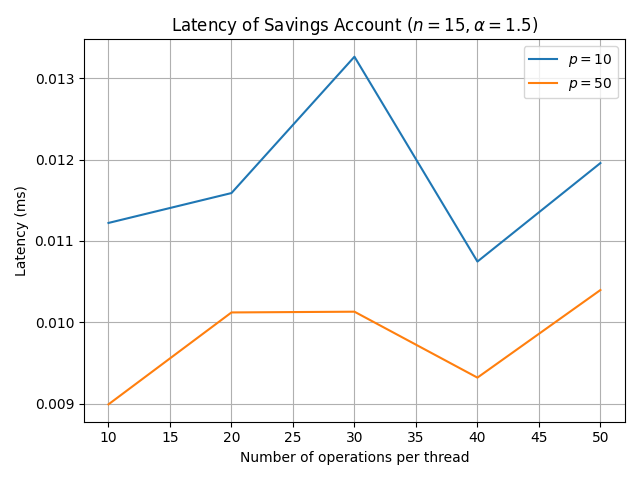
\includegraphics[width=\columnwidth]{images/exp2.png}
    \caption{Latency vs. Number of operations per thread.}
    \label{fig:exp2}
\end{figure}

\subsection{Latency vs. Number of Accounts}
As observed in the previous experiments, we expect latency to be reduced as the
number of accounts increase since the same number of threads can operate more
accounts and are less likely. Thus, there are fewer waits on condition
variables, which improves throughput. The results are shown in
\autoref{fig:exp3}.

\begin{figure}[!ht]
    \centering
    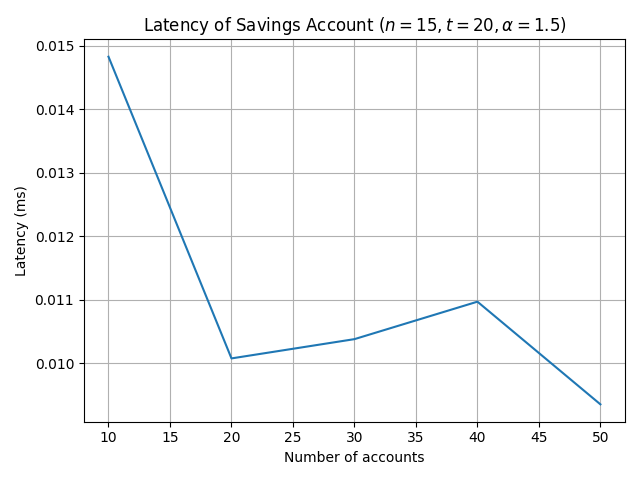
\includegraphics[width=\columnwidth]{images/exp3.png}
    \caption{Latency vs. Number of operations per thread.}
    \label{fig:exp3}
\end{figure}

\section{Challenges}

Below, we list the various challenges faced during implementation.
\begin{enumerate}
    \item Since locks and condition variables are used within the
    \texttt{SavingsAccount} class, we could not create a \texttt{SavingsAccount}
    object using the default constructor as that is deleted. The reason for this
    is that the locks and condition variables are not copyable. We fixed it by
    creating an array of pointers to the \texttt{SavingsAccount} objects,
    created using \texttt{std::make\_unique}. Threads use these pointers to
    access the object.
    \item There were instances where threads block forever due to insufficient
    funds. Since the amounts chosen are random, it is possible that a withdrawal
    blocks indefinitely and there is no deposit after. This would prevent the
    thread from being joined. To fix this, we simply introduced a large enough
    starter balance in every account.
\end{enumerate}
\end{document}